\section{Exploration of focal areas}

In addition to working with the 24 large GBRMPA regions and water bodies, it is possible to define
very specific spatial and temporal domains that might represent areas of greater focus.  For
example, it might be of interest to model water quality patterns in a defined area proximal to a
source of river discharge as part of an exploration into water quality responses to catchment
outcomes.

Small spatial domains also presents an opportunity to explore data assimilation options.  The current
project has access to four streams of water quality data (discrete AIMS niskin samples, AIMS FLNTU
data, Satellite remote sensing and eReefs modelled data).  Assimilating eReefs data (4km resolution)
and Satellite data (1km resolution) as presented in the eReefs model data represents substantial
computational overheads as a result of their high dimensionality.  Whilst the discrete AIMS niskin
sample is substantially more sparse, it does nonetheless present its own challenges when it comes to
assimilation (see below).
 
We have three choices for combining the discrete AIMS niskin sample data with the eReefs assimilated
model data:
\begin{enumerate}
\item aggregate together the average discrete (Niskin) sample and the average eReefs data
or indices.
\item assimilate via an Ensemble Kalman Filter similar to the eReefs/Satellite data assimilation
\item define a Gaussian Process that incorporates both the discrete AIMS niskin data and eReefs
  assimilated data
\item assimilate via Fixed Rank Kriging 
\end{enumerate}

As a motivating example, we will use the discrete AIMS niskin and eReefs model data surrounding a
single Dry Tropics Midshelf AIMS MMP site (Yongala).  Yongala is a deep water site and thus the
eReefs and discrete AIMS niskin samples are likely to have been collected across a relatively
homogeneous bathymetry.  Initial discussions will focus only on data from a single day (25/03/2017).
The spatial configuration of eReefs observations relative to the AIMS MMP Yongala niskin sampling
location is displayed in Figure \ref{fig:focalArea_Spatial.Yongala_Measure.chl}. 

\begin{figure}[!hptb]
  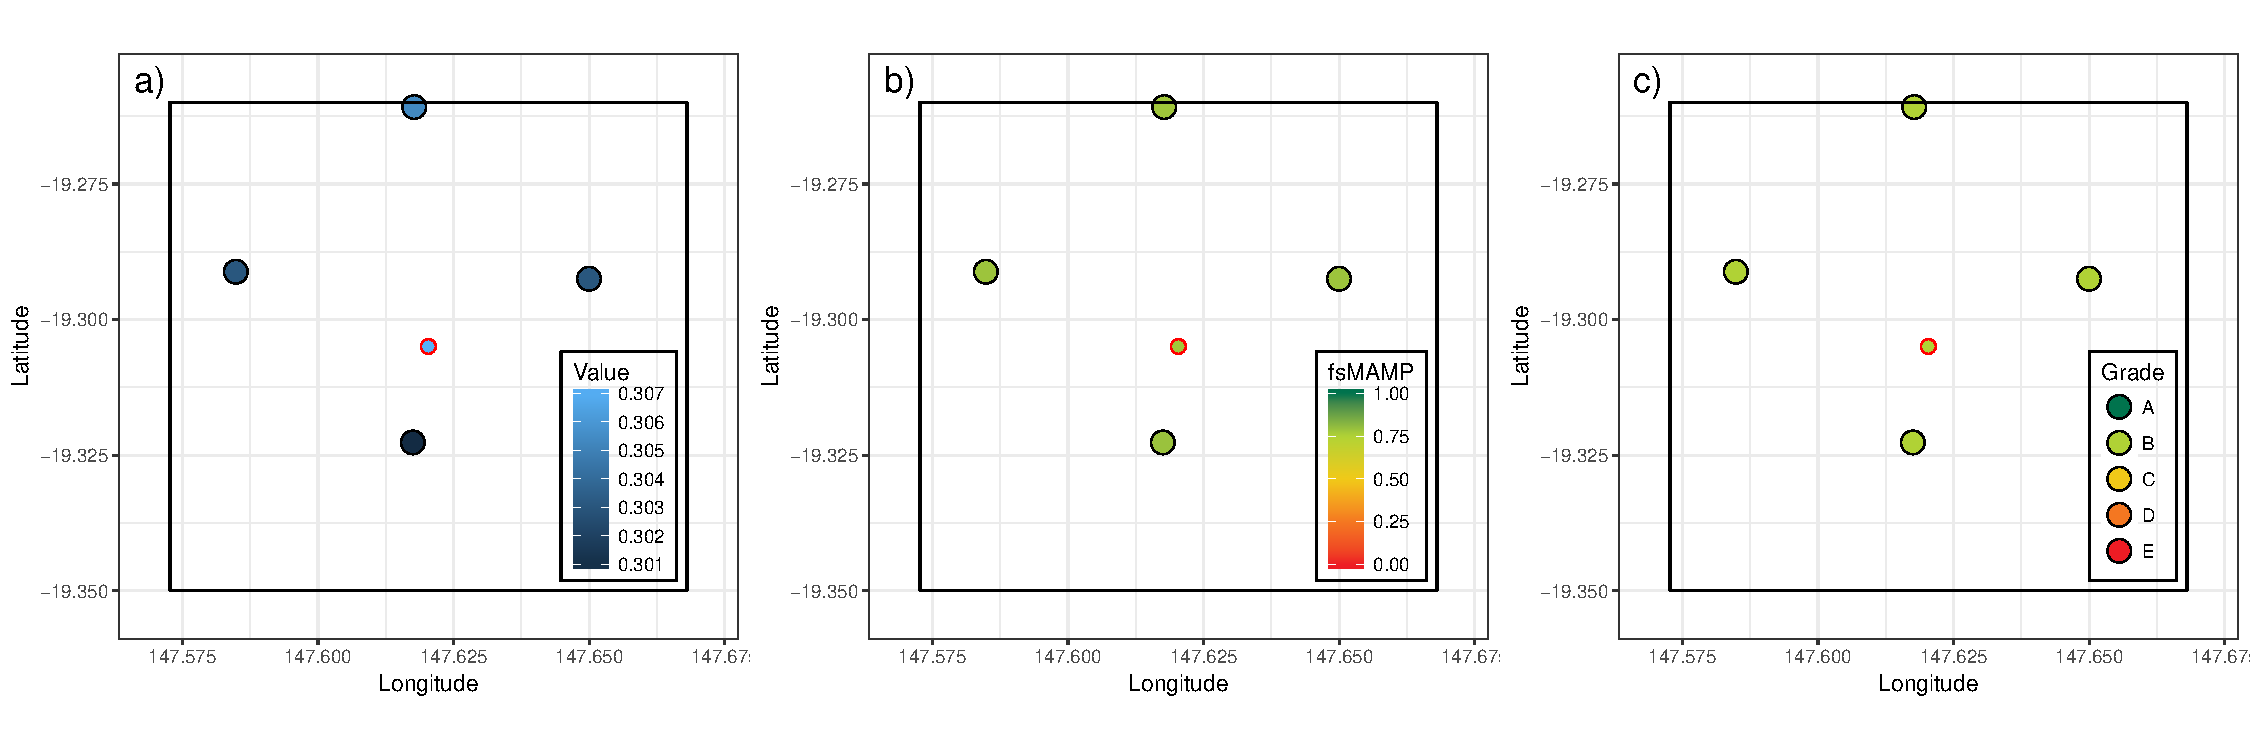
\includegraphics[width=\textwidth]{figures/FocalAreas/focalArea_Spatial.Yongala_Measure.chl.pdf}
    \caption{Spatial distribution of eReefs observation locations within 5km of the Yongala AIMS MMP niskin sampling location (point with red outline).  Observations represent a) Chlorophyll-a values and associated b) fsMAMP indices and c) Grades (Uniform control chart) for 25/03/2015.}\label{fig:focalArea_Spatial.Yongala_Measure.chl}
\end{figure}

Importantly, although the AIMS niskin sample is located geographically roughly in the middle of the
eReef locations, its Chlorophyll-a value (and fsMAMP index) is higher (and lower) than the surrounding
eReefs values.  Although this is only subtle in this example, it will be drawn upon when discussing
aggregation options.

The fact that the observed AIMS niskin Chlorophyll-a sample collected on 25/03/2015 is
higher than the surrounding eReefs estimates might suggest that either or both observation
sets are only representative of limited scales.  More specficially, it is likely that whilst the
AIMS niskin samples only acurately reflect very local conditions, the 4km eReefs data are
only likely to be reflective of broad larger scale conditions\footnote{The eReefs observations represent
  average modelled conditions within a 4x4km square cell, and therefore whilst potentially broadly reflective
  of large scale conditions, may not actually be an acccurate reflection of anywhere in that 4x4km cell}.

The above situation is likely to be exacerbated in highly heterogeneous seascapes.
AIMS niskin
samples are typically collected in close proximity to coral reefs where the general hydrology
and input process might be substantially different to the surrounding deeper water.  By contrast,
the eReefs model is known to be less reliable in shallow water.  Thus, in areas that are
heterogeneous with respect to bathymetry and hydrology, the AIMS niskin observations are
likely to be representative of only the immediate vicinity (with very similar hydrology etc),
whereas the eReefs observations might represent 'average' conditions that are only appropriate
when considered on relatively large scales. The 4km resolution of eReefs model is unlikely to present adequate granuality in areas that
are heterogeneous with respect to bathymetry and hydrology

Hence, the scale incompatibilities are likely to limit the ability to combine these two
sources of data in a meaningful and reliable manner.

It is also possible that the accuracy of the two sources differ.  Unfortunately, in the
absence of a 'truth' this is difficult to assess.  Nevertheless, since the eReefs data
are indirect measures, it is possible that they are not as accurate as the AIMS niskin
observations.  If we had co-located observations (observations collected at the same locations and
times from each source), we could attempt to align or calibrate the sources to one another.
However, it is not possible to perform such alignments when data are not co-located and there
is suspected differences in their spatial representation envelopes.

\subsection{Simple aggregation}

If we initially ignore all temporal aspects of the data and focus on the single day (25/03/2015),
we could aggregate together the single discrete AIMS Niskin sample observation with the average of the four
eReefs observations to yeild a single Chlorophyll-a estimate for the Yongala focal area  (see Figure \ref{fig:focalArea_Spatial.Yongala_Measure_Method1.1.chl}a).  Alternatively,
we could aggregate Chlorophyll-a indicies (see Figure \ref{fig:focalArea_Spatial.Yongala_Measure_Method1.1.chl}b-c).

\begin{figure}[!hptb]
  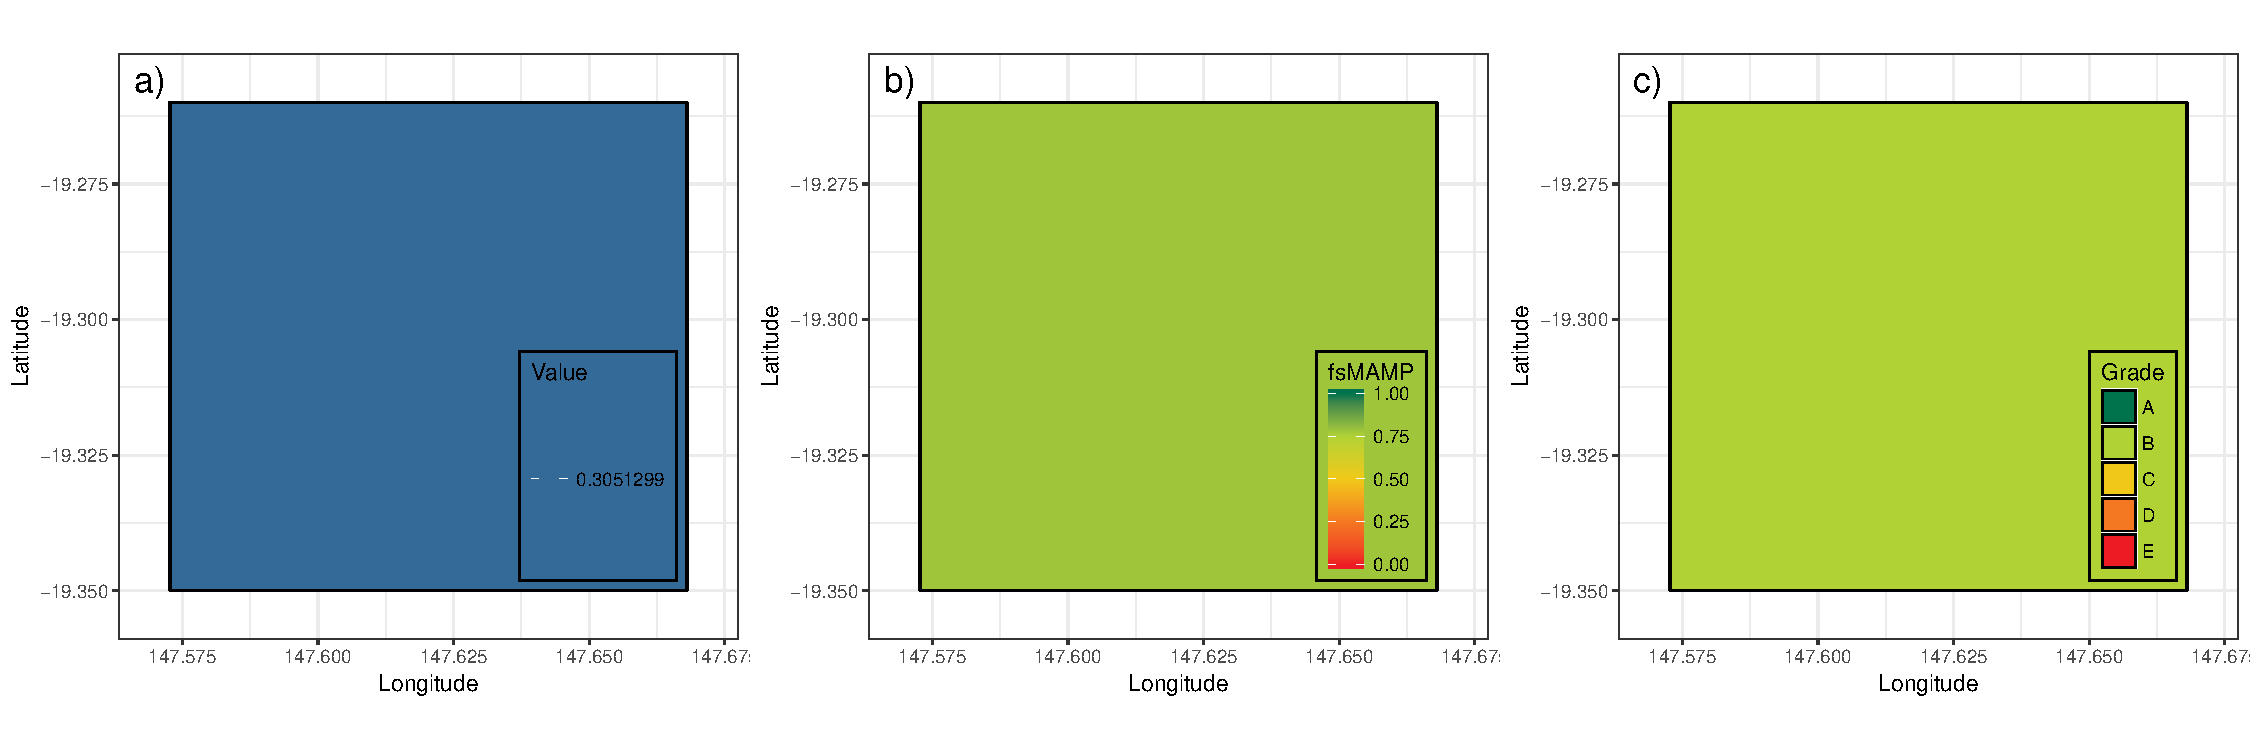
\includegraphics[width=\textwidth]{figures/FocalAreas/focalArea_Spatial.Yongala_Measure.chl_Method1.1.pdf}
    \caption{Yongala focal area aggregated a) Chlorophyll-a values and associated b) fsMAMP indices and c) Grades (Uniform control chart) for 25/03/2015.}\label{fig:focalArea_Spatial.Yongala_Measure_Method1.1.chl}
\end{figure}

Critically, this technique does assume that 
the single discrete AIMS niskin sample is representative of
the entire spatial domain of the Yongala focal area.  That is, we assume that the
focal area mean is equal to this single point estimate. 
As previously discussed, this is likely to be an unrealistic expectation.  We currently do not have any information
on the spatial envelope represented by discrete samples.
It is highly likely that the discrete samples are
spatially biased (unrepresentative of the broader area as they are typically designed to sample
reefs rather than the general water body.  Rather it is likely that the discrete sample only
represent the immediate vicinity and uncertainty should decline with increasing distance.  That
said, the form to which certainty (representation) declines is completely unknow making it
impossible to incorporate.

Furthermore, for the purpose of propagating uncertainty, the spatial uncertainty 
associated with the AIMS niskin sample is assumed to remain constant throughout this focal area.
That is, our confidence in the focal mean is informed purely in our confidence in the
single observation and that there is no additional loss of confidence associated with
increasing distance from the sampling location.
Obviously, it is highly unlikely that the reliability of the estimate will remain constant.
The same is true for eReefs data, although it is likely to be less of an issue due to the greater sample size and spatial extent.

\subsection{Ensemble Kalman Filter data assimilation}

This is the approach used to assimilate
the Satellite data into the eReefs model.
Data Assimilation (DA) is a technique with forecasting and reanalysis, the latter of
which involves conditioning estimates of state on multiple sources
of data.
For example, high density modelled data based on thermodynamics and gas laws might be
'calibrated' or augmented by data observed at weather stations.
The Kalman filter estimates state as the joint probability
distribution ($p(x|y)$) which according to Bayes rule is proportional to
the prior probaility ($p(x)$) multiplied by the probability (likelihood) of
the observational data ($p(y|x)$).
The simple Kalman filter provides algebraic expressions that
describe the transition of state mean and covariance over time
assuming all probability density functions are Gaussian and the
transition is linear.
If we say we have a prior belief that the state ($x$) has a mean of
$\mu$ and covariance of $Q$ and that the data ($d$) have an expected
value of $Hx$ and covariance of $R$, it can be shown that the posterior
mean ($\hat{\mu}$) and covariance $\hat{Q}$ are:\\

$$\hat{\mu} = \mu + K(d - Hx), \hat{Q} = (I - KH)Q$$\\

where $K$ (the Kalman gain) is:\\

$$K = QH^T(HQH^T + R)^{-1}$$

Unfortunately, as the domain of $x$ increases (higher dimensionality), the
covariance becomes prohibitatively large.
If however, the state space ($x$) is broken up into a series of
states (each perhaps representing a small subset (or ensemble) over time/space),
we can replace $Q$ with $C$ (the sample covariance).

In either case, we must have estimates of both $C$ and $R$.  Whilst
we can obtain estimates of $C$, estimates of $R$ are not possible.  If
we only have a single discrete value within a higher-dimensional
model domain, then we have no way of estimating $R$.  Furthermore,
even in larger focal areas that might contain multiple discrete
samples, the samples are too spread out both spatially and
temporally to be able to estimate $R$ with any accuracy or
reliability.  For example, whilst the samples are typically
separated in space by 10's of kilometers and months in time, water
samples are likely to vary over the scale of meters and hours.


\subsection{Gaussian Processes}

A Gaussian distribution represents the distribution of observations that are themselves the result of an infinite number of influences (or processes).
They are widely used to represent the distribution of residuals (unexplained component) when modelling data as it is often assumed that the
unexplained component is due to a huge number of additional, unmeasured influences.  In traditional linear modelling, we assume that not only
are the residuals normally (Gaussian) distributed, we also assume that they are independent (not spatially or temporally correlated) and equally
varied around 0.

$$
\varepsilon_i \sim~\mathcal{N}(0, \Sigma)\hspace{1cm}
\Sigma = 
\begin{pmatrix}
\sigma^2 &   0      & \ldots   & 0\\
0        &\sigma^2  & \ldots   & \vdots\\
\vdots   & \ldots   &\sigma^2  & \vdots\\
0        & \ldots   &\ldots    &\sigma^2
\end{pmatrix}
$$

Similarly, rather than express the stochastic elements as a vector of residuals drawn from a normal distribution, we can
model the observed data as a multivariate normal (Gaussian) distribution.  In this case, we are assuming that each of the
observations is drawn from a multivariate normal distribution with different means and covariances).

This same argument could be extended to describe the distribution from which functions are drawn.  
Observed data are the result of the sum of an in infinite number of processes (including measurement error).  Many of these processes
vary over space and time such that sampling units that are closer together in space and time tend to be more similar to one
another than they are to more distant units.


$$
y_i \sim~\mathcal{MVN}(M, C)\hspace{1cm}\\
$$

A Gaussian Process is largely defined by the covariance matrix ($k(x,x^\prime)$).  Actually $k$ is referred to as the \textbf{kernel}.
We can define any covariance (kernel) function provided it is semi-definite - essentially that it is a symmetrical matrix.

A few of the popular kernels are described in the following Table \ref{ref:GP_functions}.

\begin{table}[!htbp]
  \caption{Simple Gaussian Process kernel functions}\label{ref:GP_functions}
  \begin{tabular}{ll}
    \toprule
    Kernel & Function\\
    \midrule
    Linear &              $k(x,x^\prime) = \sigma^2_f xx^\prime$\\[1em]
    Squared exponential & $k(x,x^\prime) = \sigma^2_f exp\left[\dfrac{-(x-x^\prime)^2}{l^2}\right]$\\[1em]
    Periodic   &          $k(x,x^\prime) = \sigma^2_f exp\left[\dfrac{-2\sin^2(\pi(x-x^\prime)/p}{l^2}\right]$\\[1em]
    Periodic exponential & $k(x,x^\prime) = \sigma^2_f exp\left[\dfrac{-2\sin^2(\pi(x-x^\prime)/p}{l_1^2}\right]exp\left[\dfrac{-(x-x^\prime)^2}{l_2^2}\right]$\\[1em]
    Matern     &          $k(x,x^\prime) = \sigma^2_f \dfrac{1}{\Gamma(v)2^{v-1}}\left[\dfrac{\sqrt{2v} |(x-x^\prime)|}{l}\right]^v K_v\left[\dfrac{\sqrt{2v} |(x-x^\prime)|}{l}\right]$\\[1em]
    \bottomrule
  \end{tabular}
\end{table}

In Table \ref{ref:GP_functions}, $x$ and $x^\prime$ are vectors of the X variable.  $x^\prime$ just indicates a transposed version of the vector.
Hence $(x-x^\prime)$ indicates the difference (distance) between each pair of x values (they are squared so that they are all positive).
When two points are similar, $k(x,x^\prime)$ approaches 1 (perfect correlation).  Smoothing is based on neighbours exerting influence on one another (being correlated).
When two points are very distant $k(x,x^\prime)$ approaches 0.
The $l$ are length scale parameters that determines the degree of contagion - that is, they determine the rate that the influence
of points deteriorates with distance.

Assuming that the covariance pattern defined by the GP parameters (e.g. $\sigma_f^2$ and $l$) and observation space reliably reflects the underlying processes,
the same parameters can be applied to yield a covariance structures for predicting mean and variance across a noval (yet overlapping) space.  Specifically, if the
covariance across the observed space is $K_{oo}$, the covariance between observed and prediction space is $K_{op}$ and the coavariance across prediction space
is $K_{pp}$, then the mean and variance for predicted values are:\\

$$
\bar{y}_p = K_{op}(K_{oo} + \sigma_o^2I)^{-1}K^T_{op}y_o$$
and 
$$var(y_p) = K_{pp} - K_{op}(K_{oo}+ \sigma_o^2I)^{-1}K^T_{op}$$

where $\sigma_o^2$ is the estimated variance (uncertainty) in the observations, $I$ is an identity matrix of equivalent dimensionality to $K_{oo}$ and $K_{op}^T$ is the transpose of $K_{op}$. 

Gaussian Processes could be used to fit smooth multidimensional smoothers separate over each source so as to estimate
parameters and uncertainty at any granulariy.  Whilst this might be appropriate for the eReefs data,  it is not possible
to build a reasonable gaussian process via a single point without external estimates of the covariance over functions ($\sigma_f^2$)
and the length (wiggliness) of the smoother.

Normally a Gaussian Process is applied to a single source for the purpose of kriging (smoothing).
Nevertheless, it could be argued that there are a single set of underlying processes driving spatio-temporal patterns of water quality (e.g. $l$ and $\sigma_f^2$)
and that the multiple sources (AIMS niskin and eReefs) represent alternative ways to sample observations from those processes.  Ideally, any differences between the sources
should purely be differences in accuracy and uncertainty.  If this is the case, rather than assume all observations are associated with the same $\sigma_o^2$, we could
asssociate one variance to the AIMS niskin observations ($\sigma_n^2$) and another to the eReefs observations ($\sigma_e^2$).

Figure \ref{fig:focalArea_Spatial.Yongala_Measure_Method2.1.chl} illustrates a squared exponential Gaussian Processes with different parameter values applied to a single dimension (Latitude) of the
25/03/2015 Yongala focal area data.  In each case, the variability (uncertainty) of the AIMS niskin observations was defined as 10 times lower than than of the eReefs observations.
Values of $\sigma_f^2$ and $l$ were chosen to represent specific sets of scenarios.  For example, lower $\sigma_f^2$ imposes a lower maximum covariance and a lower $l$ dictates are
more rapid decline in the autocorrelation over distance.  Whilst it is possible to apply these functions in an optimizing framework so as to allow the data to determine
the most appropriate values for $\sigma_f^2$ and $l$, $\sigma_n^2$ and $\sigma_e^2$ must be supplied based on external estimates.   

\begin{figure}[!hptb]
  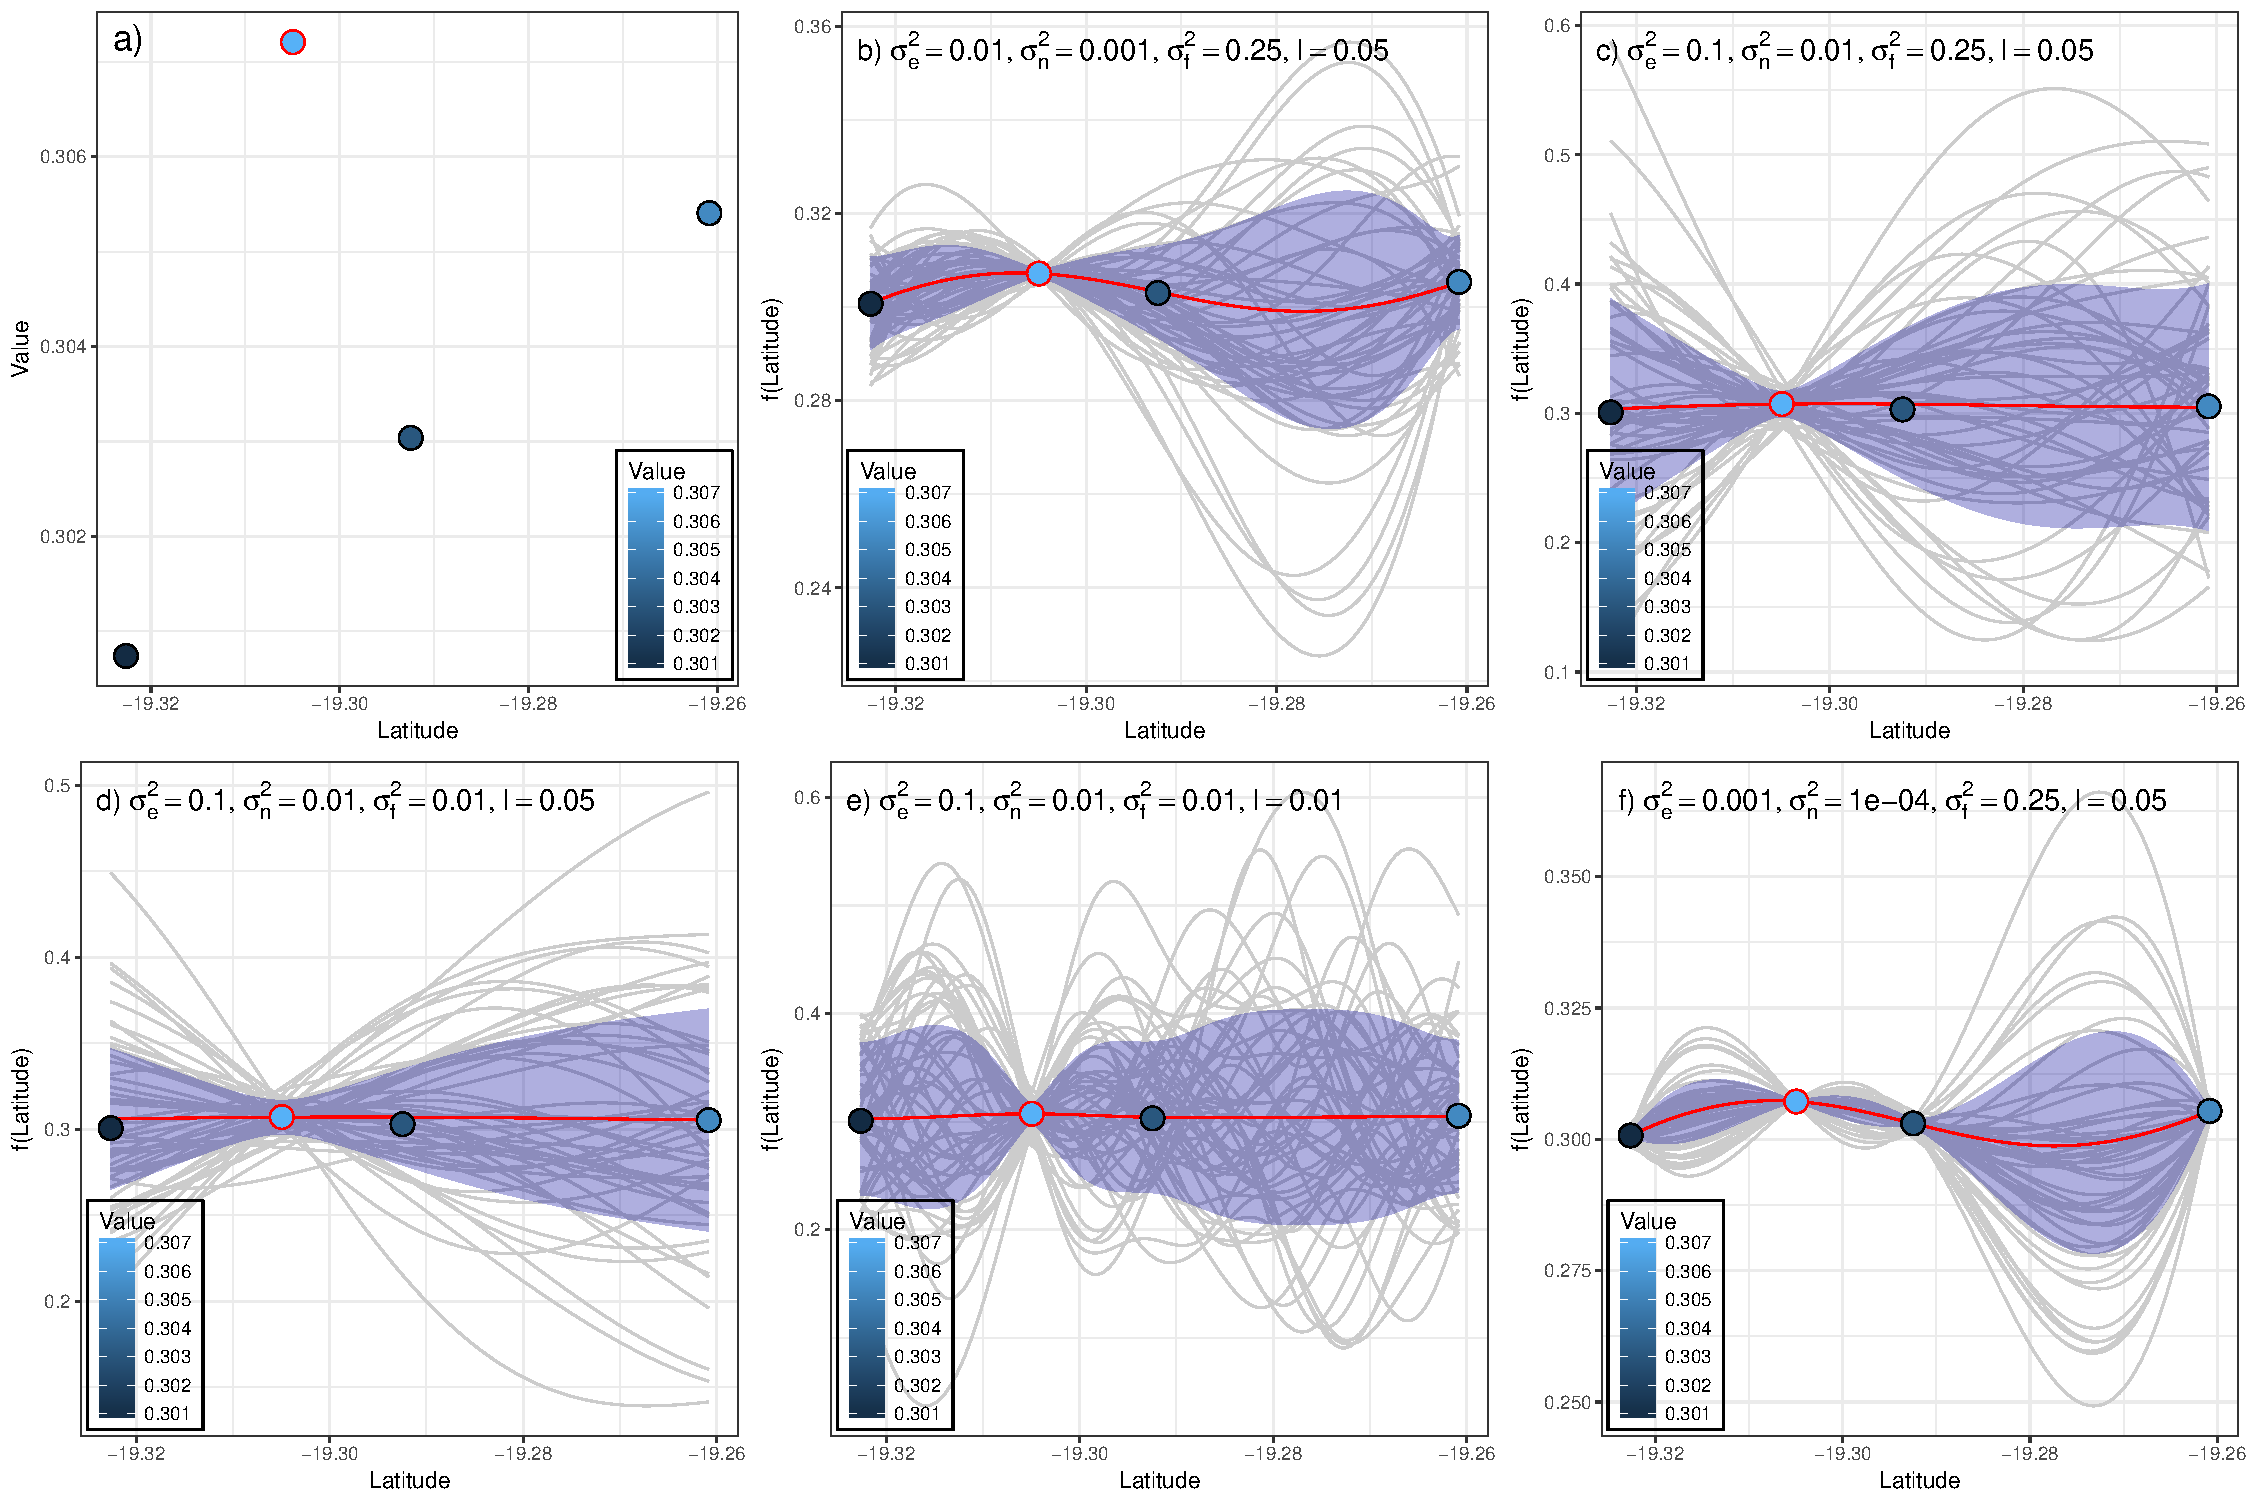
\includegraphics[width=\textwidth]{figures/FocalAreas/focalArea_Spatial.Yongala_Measure.chl_Method2.1.pdf}
  \caption{Illustration of data assimilation via squared exponential Gaussian process applied to a single dimension (Latitude) for the 25/03/2015 Yongala focal area a) Raw Chlorophyll-a values and b-e) different Gaussian Process parameters.}\label{fig:focalArea_Spatial.Yongala_Measure_Method2.1.chl}
\end{figure}
  
Similar to the Kalman Filter, high dimensionality incurs substantial covariance size increases.
Every one additional observation results in a doubling of the covariance matrix and a tripling of
memory to invert this the covariance matrix.  Hence, practical applications employ either ensemble-like approaches
or more commonly, sparse covariance matrices\footnote{Sparse matrices acknowledge that covariance will decline over time and distance and at some distance, the covariance will effectively be zero.} to reduce the imposition of dimensionality.

Addition of a temporal dimension substantially increases the complexity of the problem.  Not only does the covariance structures have to account for variability and autocorrelation length
over space, it also has to reflect patterns of variability over time.  Importantly, it is not just how isolated spatial points change over time.  Temporal autocorrelation also occurs between
neighbouring points.


\subsection{Fixed Rank Kriging}

Fixed Rank Griging (FRK) is a spatio-temporal modelling and prediction framework
in which spatially/temporally correlated random processes are decomposed via
linear combinations of basis functions ($\boldsymbol{\Phi}$) along with associated fine-scale variation ($\boldsymbol{\nu}$) \citep{Cressie-2008-209}.

$$
\boldsymbol{Y} = \mathbold{X}\boldsymbol{\beta} + \boldsymbol{\Phi}\boldsymbol{\alpha} + \boldsymbol{\nu}
$$

The use of relatively small numbers of basis functions permits substantial dimensionality reductions that offers
a scalable solution for very large data sets.  Moreover, the framework facilitates differing spatial support hence allowing
some capacity for the 'fusion' of multiple sources with different footprints.

%The varying footprints of the two data sources (AIMS niskin and eReefs modelled data) are 
Varying footprints are accomodated by arranging the point-referenced data into grids,
the granularity of which is proportional to the footprint or extent of support.  For example,
the AIMS niskin data and eReefs modelled data could be descretized into a small and set of larger
grid squares (see Figure \ref{fig:focalArea_Spatial.Yongala_Measure.chl_Method3}b - pale red and blue squares respectively).
Whilst the footprint size for the eReefs modelled data was based on the cell grid onto which the model
is projected, the AIMS niskin footprint was set to an arbitrarily (smaller) value to illustrate varying
degrees of support.

The full spatio-temporal domain is also discretized into a regular grid of smaller cells called
\textit{basic areal units} (BAU) which represent the smallest modelling and prediction unit.
In this example, we have discretized the spatial domain by hexagonal cells 0.01 degrees longitude by 0.01 degrees latitude (see Figure \ref{fig:focalArea_Spatial.Yongala_Measure.chl_Method3}b - black hexagons).
Within the model, varying support is then based on the intersection of the square footprints with
the BAUs.

For this example, we have elected to define two regularly spaced basis functions based on Matern covariance (smoothing parameter of 1.5)
to be used in the decomposition of spatio-temporal processes (see Figure \ref{fig:focalArea_Spatial.Yongala_Measure.chl_Method3}c).
The multiple resolutions provide a mechanism
for esimating the scale of spatio-temporal autocorrelation (however, ideally this requires a substantially
larger grid of data than our example).

The basis function covariance matrices and fine-scale variance parameters are estimated via a expectation maximization (EM)
algorithm and thereafter used to project predictions onto the scale of the BAU's (see Figure \ref{fig:focalArea_Spatial.Yongala_Measure.chl_Method3}d).
These predicted values have also been indexed via fsMAMP (see Figure \ref{fig:focalArea_Spatial.Yongala_Measure.chl_Method3}e) and
converted into Grades (see Figure \ref{fig:focalArea_Spatial.Yongala_Measure.chl_Method3}f).

\begin{figure}[!hptb]
  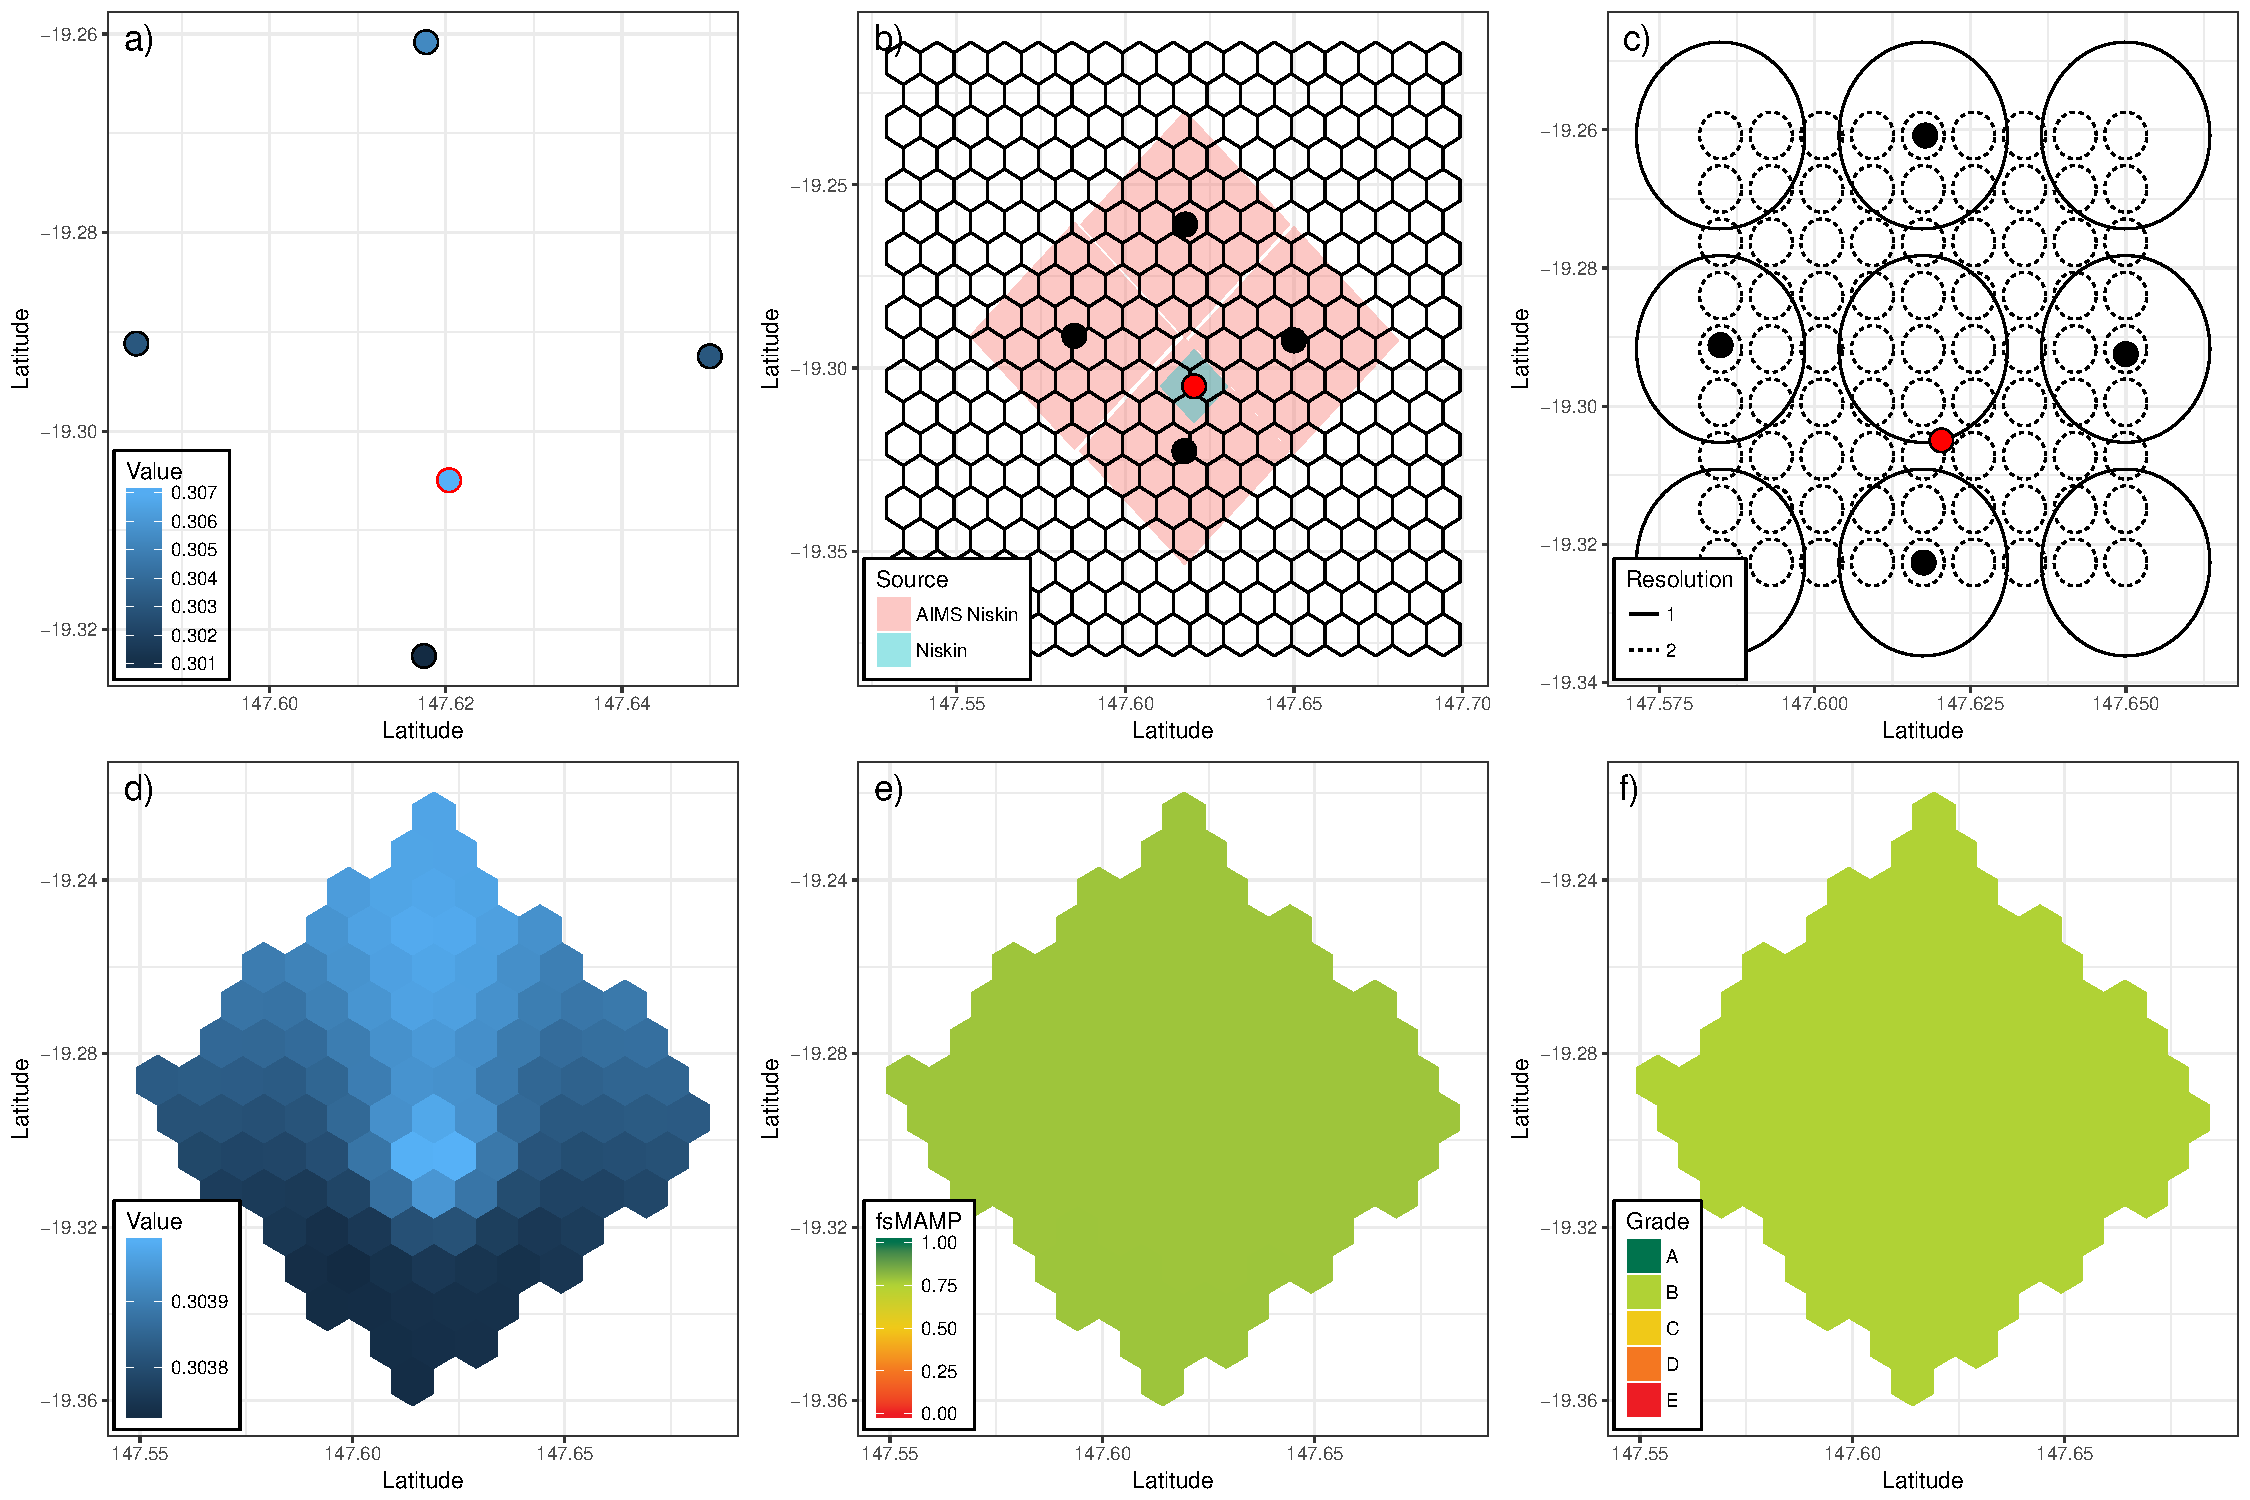
\includegraphics[width=\textwidth]{figures/FocalAreas/focalArea_Spatial.Yongala_Measure.chl_Method3.pdf}
    \caption{Illustration of data assimilation via Fixed Rank Kriging applied to spatial data for the 25/03/2015 Yongala focal area a) Raw Chlorophyll-a values (AIMS niskin: red symbol border, eReefs: black symbol border), b) dicretization of the spatial domain into a regular hexagonal grid and varying footprints (support) for AIMS niskin (blue) and eReefs (red), d) Matern basis functions of two resolutions, d) predicted values and associated e) fsMAMP indices and f) Grades (Uniform control chart) for 25/03/2015.}\label{fig:focalArea_Spatial.Yongala_Measure.chl_Method3}
\end{figure}

Figure \ref{fig:focalArea_Spatial.Yongala_Measure.chl_Method3} illustrates that whilst fixed rank kriging does offer
an option for the assimilation (or fusion) of multiple data sets, in the absence of measurement error,
it does assume that all observations are equally accurate.  Figure \ref{fig:focalArea_Spatial.Yongala_Measure.chl_Method3}d
shows a bright spot associated with the higher AIMS niskin Chlorophyll-a value.
It is important to reiterate that the extent of this bright spot is due to both the higher Chlorophyll-a observation
of the AIMS niskin sample and the arbitrary size of the footprint.  To be a meaningful fusion, reasonable
estimates of the spatio-temporal extent of representation of the AIMS niskin data will need to be obtained along
with estimates of measurement error in both the AIMS niskin and eReefs modelled data.

Spatio-temporal basis functions can be constructed as the tensor product of spatial basis functions and
similarly defined temporal basis functions.  Measurement error (if known) can also be incorporated.

More recently, \citet{Nguyen-2014-175} has proposed a data assimilation technique for big data that is
essentially a blend of fixed rank kriging and Kalman filtering and looks to have some promise.